\documentclass[12pt,a4paper,twoside]{article}
\usepackage[a4paper, total={7in, 10in}]{geometry}
\usepackage[backend=biber]{biblatex}

\usepackage{listings}   %configuration for codes
\usepackage{colortbl}

\definecolor{codegreen}{rgb}{0,0.6,0}
\definecolor{codegray}{rgb}{0.5,0.5,0.5}
\definecolor{codepurple}{rgb}{0.58,0,0.82}
\definecolor{backcolour}{rgb}{1.0,1.0,1.0}

\lstdefinestyle{plain}{
	backgroundcolor=\color{backcolour},   
	numberstyle=\tiny\color{codegray},
	basicstyle=\ttfamily\scriptsize,
	breakatwhitespace=false,         
	breaklines=true,                 
	keepspaces=true,                 
	numbers=left,       
	numbersep=5pt,                  
	showspaces=false,                
	showstringspaces=false,
	showtabs=false,                  
	tabsize=2
}

\lstdefinestyle{Terminal}{
	language=bash,
	backgroundcolor=\color{backcolour},   
	commentstyle=\color{codegreen},
	keywordstyle=\color{magenta},
	numberstyle=\tiny\color{codegray},
	stringstyle=\color{codepurple},
	basicstyle=\ttfamily\scriptsize,
	breakatwhitespace=false,         
	breaklines=true,                 
	keepspaces=true,                 
	numbers=left,       
	numbersep=5pt,                  
	showspaces=false,                
	showstringspaces=false,
	showtabs=false,                  
	tabsize=2
}

\lstdefinestyle{CStyle}{
	language=C,
	backgroundcolor=\color{backcolour},   
	commentstyle=\color{codegreen},
	keywordstyle=\color{magenta},
	numberstyle=\tiny\color{codegray},
	stringstyle=\color{codepurple},
	basicstyle=\ttfamily\scriptsize,
	breakatwhitespace=false,         
	breaklines=true,                 
	keepspaces=true,                 
	numbers=left,       
	numbersep=5pt,                  
	showspaces=false,                
	showstringspaces=false,
	showtabs=false,                  
	tabsize=2
}

\begin{document}
\cleardoublepage
	\clearpage
\chapter{Lexical analyzer for C language using C language}

\section{Aim}
To design and implement a lexical analyzer for given language using C. The lexical analyzer should ignore redundant spaces, tabs and new lines.

\section{Algorithm}

\begin{figure}[H]
	\centering
	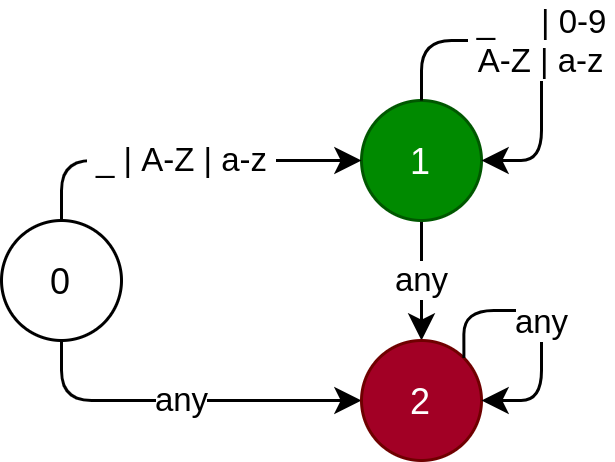
\includegraphics[height=2.5in]{../EXP1/identifier.png}
	\caption{Finite Automaton to detect an identifier.}
\end{figure}

\begin{figure}[H]
	\centering
	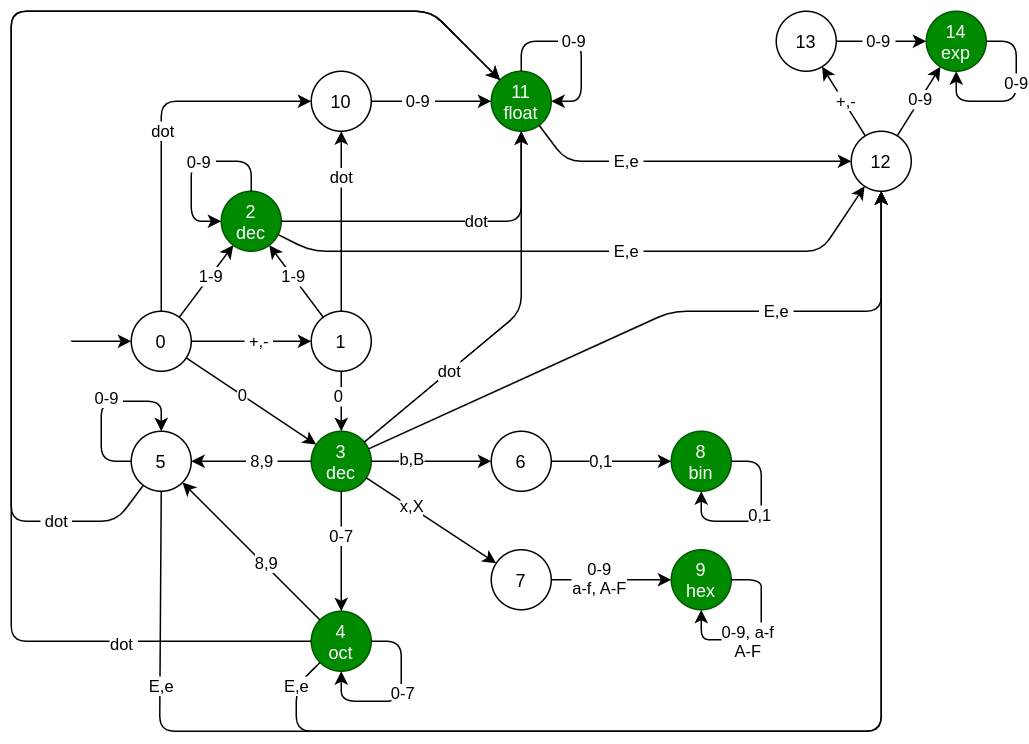
\includegraphics[width=\textwidth]{../EXP1/numerals.png}
	\caption{Finite Automaton to detect an numeral type.}
\end{figure}


\begin{figure}[H]
	\centering
	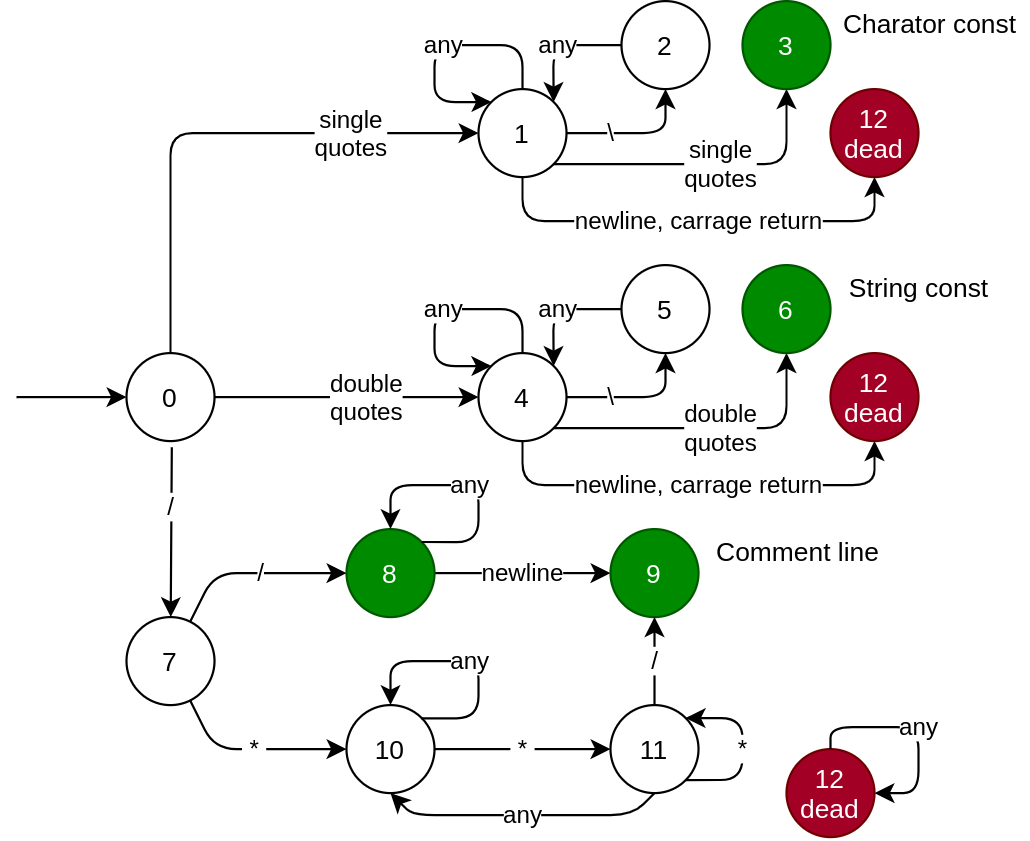
\includegraphics[width=\textwidth]{../EXP1/char-stream.png}
	\caption{Finite Automaton to detect comments, string/char literal and escape sequence}
\end{figure}


\section{C-Program}
Header file \textbf{stack.h} to stimulate stack.
\lstinputlisting[style=CStyle]{../EXP1/stack.h}

\vspace{0.5cm}
Header file \textbf{definition.h} holds various subroutines and constants that aid to analyze lexemes of C language.
\lstinputlisting[style=Cstyle]{../EXP1/definition.h}

\vspace{0.5cm}
C program file \textbf{CLexical.c} initiates and scans lexemes.
\lstinputlisting[style=Cstyle]{../EXP1/CLexical.c}


\section{Output}
C program used for testing \textbf{sample.c}.
\lstinputlisting[style=CStyle]{../EXP1/sample.c}

\vspace{0.5cm}
Lexical analyzer output
\lstinputlisting[style=plain]{../EXP1/sample_out.txt}

\section{Result}
The program compiled successfully and identified various C tokens from the sample C program file.
	 
	\cleardoublepage
	\clearpage
\chapter{Lexical analyzer for C language using Lex tool}

\section{Aim}
To design and implement a lexical analyzer for given C language using lex tool. The lexical analyzer should ignore redundant spaces, tabs and new lines.

\section{Algorithm}

\begin{figure}[H]
	\centering
	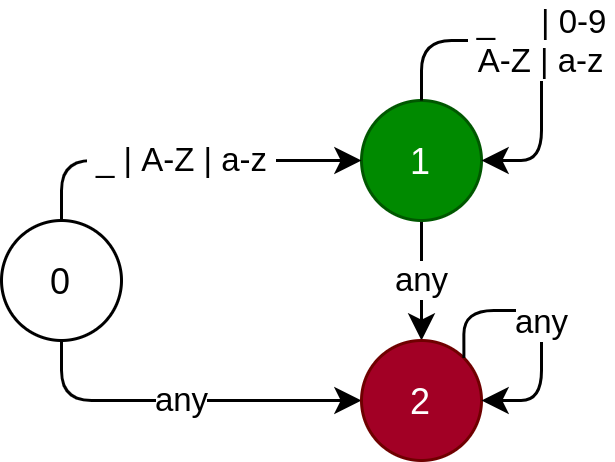
\includegraphics[height=2.5in]{../EXP1/identifier.png}
	\caption{Finite Automaton to detect an identifier.}
\end{figure}

\begin{figure}[H]
	\centering
	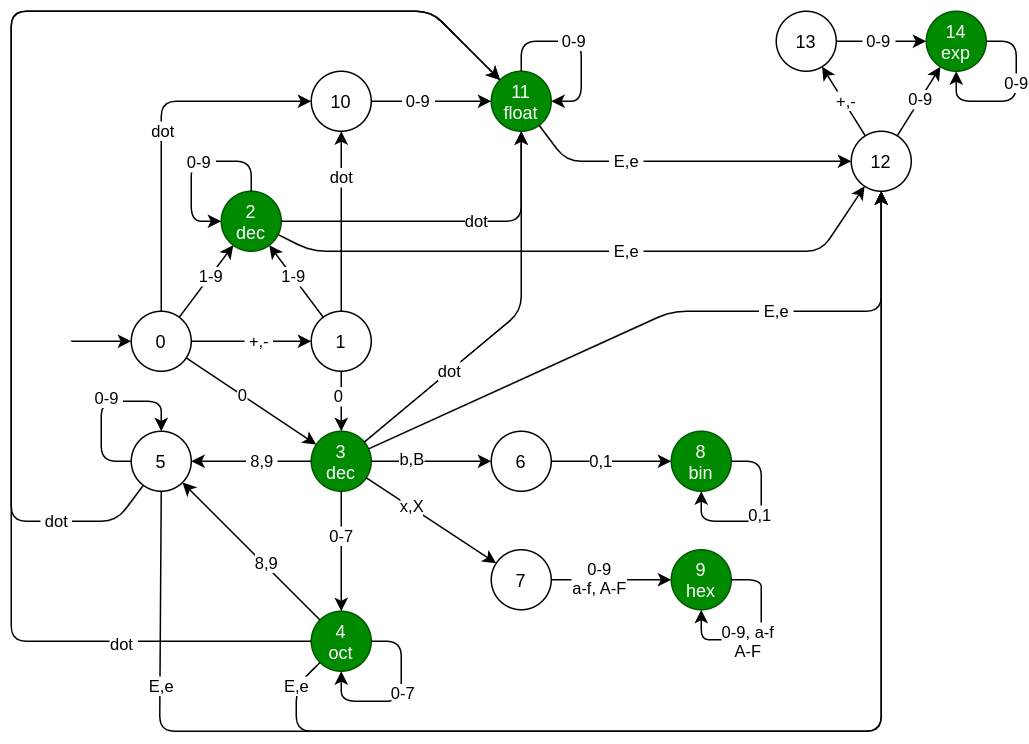
\includegraphics[width=\textwidth]{../EXP1/numerals.png}
	\caption{Finite Automaton to detect an numeral type.}
\end{figure}


\begin{figure}[H]
	\centering
	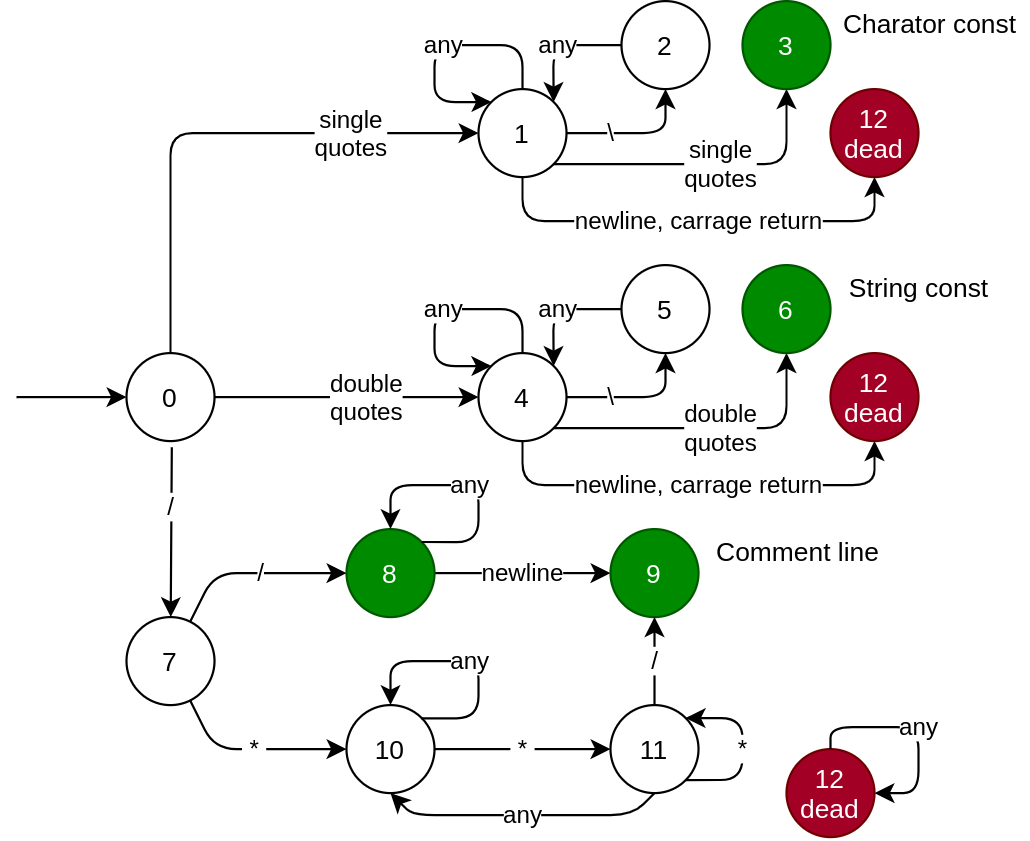
\includegraphics[width=\textwidth]{../EXP1/char-stream.png}
	\caption{Finite Automaton to detect comments, string/char literl and escape sequence}
\end{figure}


\section{C-Program}
Header file \textbf{stack.h} to stimulate stack.
\lstinputlisting[style=CStyle]{../EXP2/stack.h}

\vspace{0.5cm}
Header file \textbf{definition.h} holds various subroutines and constants that aid to analyze keywords and identifiers. The lex tool detects identifers. A table is cross checked to detect keywords.
\lstinputlisting[style=Cstyle]{../EXP2/definition.h}

\vspace{0.5cm}
Lex file \textbf{CLexical.l} initiates and scans lexemes.
\lstinputlisting[style=Cstyle]{../EXP2/CLexical.l}



\section{Output}
C program used for testing \textbf{sample.c}.
\lstinputlisting[style=CStyle]{../EXP2/sample.c}


\vspace{0.5cm}
Compiling lex file
\begin{lstlisting}[style=Terminal]
	$ lex CLexical.l
	$ gcc lex.yy.c
	$ ./a.out sample.c
\end{lstlisting}

\vspace{0.5cm}
Lexical analyser output
\lstinputlisting[style=plain]{../EXP2/sample_out.txt}

\section{Result}
The Lexicial analyser is stimulated successfully and the output is verified.
	
	\cleardoublepage
	\clearpage
\chapter{Generation of YACC specification for a few syntactic categories}

\section{Aim}
To design and implement YACC specification for the following syntactic categories.
\begin{enumerate}
	\item Program to recognize a valid arithmetic expression that uses operator +, – , * and /.
	%\item Program to recognize a valid variable which starts with a letter followed by any	number of letters or digits.
	%\item Implementation of Calculator using LEX and YACC
	%\item Convert the BNF rules into YACC form and write code to generate abstract syntax tree
\end{enumerate}


\section{Recognize Arithmetic expression}
\subsection{Algorithm}
\begin{algorithm}[H]
	\caption{An algorithm to recognize numbers , operators and variables}
	\begin{algorithmic}[1]
		\State $isNum \gets False$
		\State $isVar \gets False$
		\State $buf \gets ""$
		\State $i \gets 0$
		\State $buf[i] \gets $ inputChar()
		\While{$buf[i]$ == whitespace}
		\State $buf[i] \gets $ inputChar()
		\EndWhile
		
		\If{ $buf[i]$ == operator }
		\State $return$ $buf[i]$,"operator"
		\ElsIf{ $buf[i]$ == '(' }
		\State $return$ $buf[i]$,"openBracket"
		\ElsIf{ $buf[i]$ == ')' }
		\State $return$ $buf[i]$,"closeBracket"
		\ElsIf{$buf[i]$ == alpha or underscore}
		\State $isVar \gets True$
		\ElsIf{$buf[i]$ == number}
		\State $isNum \gets True$
		\Else
		\State $return$ "ERROR"
		\EndIf
		\State $i \gets i+1$
		
		\While{$(buf[i]$ = inputChar()) $\neq$ EOF}
		\If{$isVar and buf[i]$ == (alphaNum or underscore)}
		\State $i \gets i + 1$
		\State continue
		\ElsIf{$isNum$ and $buf$ == number)}
		\State $i \gets i + 1$
		\State continue
		\Else
		\State unputChar($buf[i]$) \Comment{Put back the last char read}
		\State $buf[i]$ = $'\ '$
		\If{$isVar$}
		\State $return$ $buf$,"variable"
		\ElsIf{$isNum$}
		\State $return$ $buf$,"number"
		\Else
		\State $return$ "ERROR"
		\EndIf
		\EndIf
		\EndWhile
	\end{algorithmic}
\end{algorithm}

\begin{algorithm}[H]
	\caption{A grammar to recognize expression}
	\begin{algorithmic}[1]
		\State $FINAL\_EXPR \gets EXPR$ $NEWLINE$
		\State $EXPR \gets number$
		\State $EXPR \gets identifier$
		\State $EXPR \gets $openBracket $EXPR$ closeBracket
		\State $EXPR \gets EXPR$ operator $EXPR$
	\end{algorithmic}
\end{algorithm}

\subsection{Lex program}
\lstinputlisting[style=CStyle]{../EXP3/expression.l}
\subsection{Yacc Program}
\lstinputlisting[style=CStyle]{../EXP3/expression.y}
\subsection{Output}
Compiling program
\lstinputlisting[style=Terminal]{../EXP3/expression_run.sh}


\vspace{0.5cm}
Output
\lstinputlisting[style=plain]{../EXP3/expression_output.txt}



\section{Result}
Implemented and verified YACC specification for a few syntactic categories
	
	\cleardoublepage
	\clearpage
\chapter{Traversing $\epsilon$ transitions in NFA}

\section{Aim}
To design and implement a C-program that accepts a Non-deterministic Finite Automaton (NFA) and computes $\epsilon$ closure for each states.

\section{Algorithm}

\begin{algorithm}[H]
	\caption{An algorithm to compute $\epsilon$ closure of a state}
	\begin{algorithmic}
		\Procedure{findEpsilionTrans}{$visited, fromState$}
		\State \Comment{visited : Stack of visited states}
		\State \Comment{fromState : Current state to find closure}
		
		\If{$fromstate \in visited$}
		\State return $visited$
		\EndIf
		
		\State $push(visited, fromState)$
		
		\ForAll{$transition \in fromState.transitions$}
		\If{$transition.symbol == \epsilon $}
		\State $visited = $ \Call{findEpsilonTrans}{visited, transition.toState}
		\EndIf
		\EndFor
		\EndProcedure
	\end{algorithmic}
\end{algorithm}

\subsubsection*{Realization of NFA using linked list}

\begin{figure}[H]
	\centering
	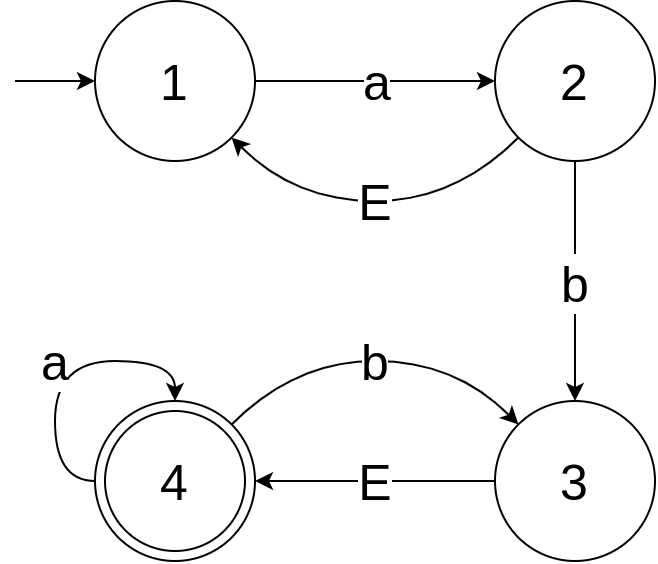
\includegraphics[height=2in]{../EXP4/NFA_realization-NFA.png}
	\caption{NFA}
\end{figure}

\begin{figure}[H]
	\centering
	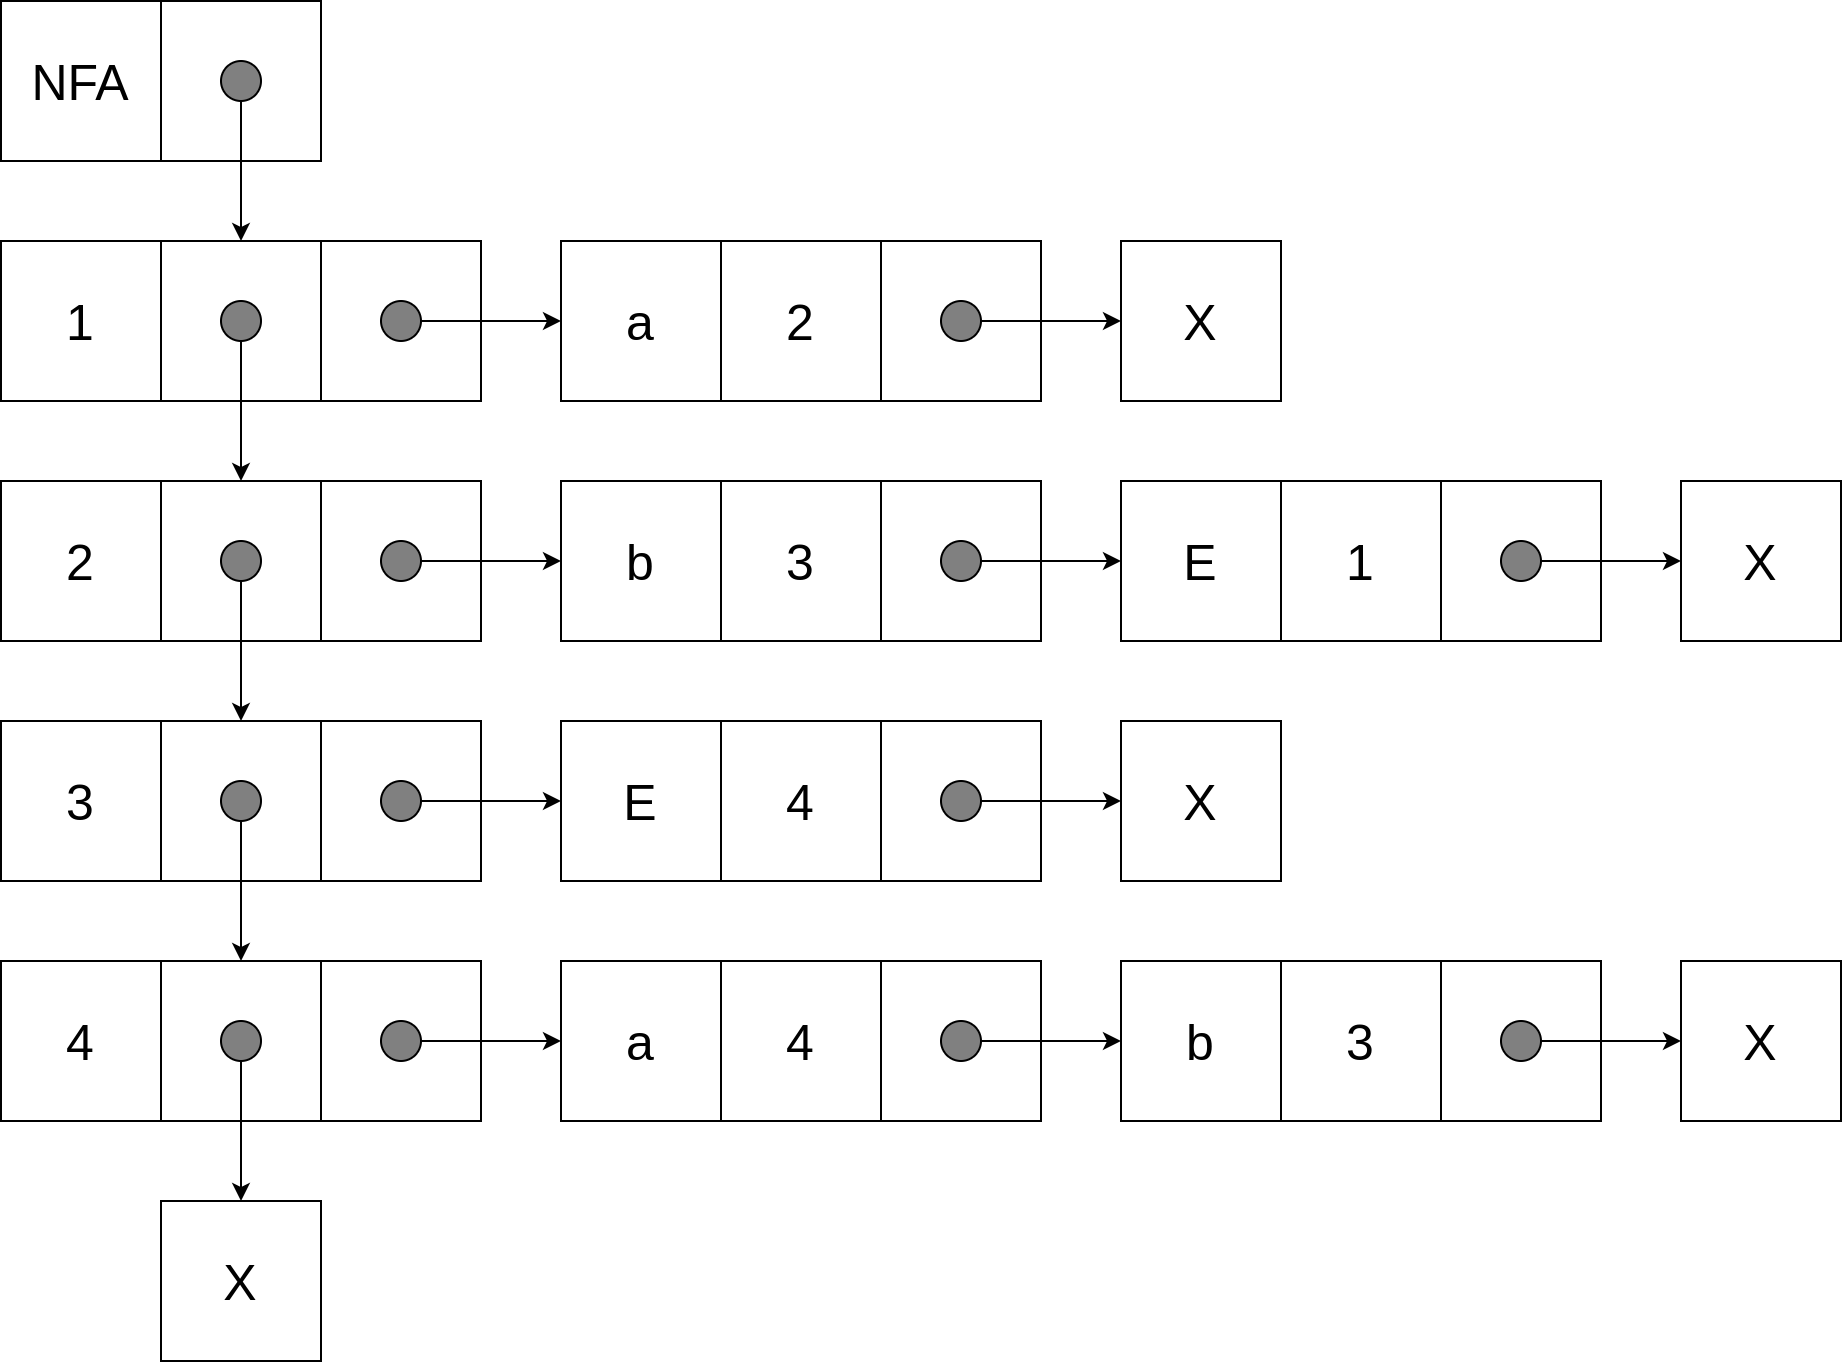
\includegraphics[height=2.5in]{../EXP4/NFA_realization-LinkedList.png}
	\caption{NFA realization via linked list}
\end{figure}
\section{C-Program}
\lstinputlisting[style=CStyle]{../EXP4/epsilonNFA.c}

\section{Output}
\lstinputlisting[style=plain]{../EXP4/output.txt}

\section{Result}
The program compiled successfully and identified $\epsilon$ closure for each states in the given NFA.
	
	\cleardoublepage
	\clearpage
\chapter{Converting $\epsilon$-NFA to NFA}

\section{Aim}
To design and implement a program that accepts a Epsilon Non-deterministic Finite Automaton ($\epsilon$-NFA) and computes NFA without $\epsilon$ transitions.

\section{Algorithm}

\begin{algorithm}[H]
	\caption{An algorithm to convert $\epsilon$-NFA to NFA }
	\begin{algorithmic}
		\Procedure{computeTransition}{$state, sym$}
			\State \Comment{state : starting state}
			\State \Comment{inputs : input symbol}
			
			\State $resultSet \gets \{\}$ \Comment{Empty set}
			
			\State $Eset \gets \Call{EClosure}{state}$ \Comment{Computing e-closure}
			
			
			\ForAll{$Estate \in Eset$}
				\State $Tstates \gets \Call{transition}{Estate,sym}$ \Comment{set of states after transition}
				\ForAll{$subState \in Tstates$}
					\State $resultSet \gets resultSet \cup \Call{EClosure}{subState}$ \Comment{Union of eclosures}
				\EndFor
			\EndFor
			\State return $resultSet$
		\EndProcedure

		\ForAll{$state \in TotalStates$}
			\State $symbols \gets \Call{getInputSymbols}{state}$ \Comment{set of possible input symbols}
			\ForAll{$sym \in symbols$}
				\State $Eset \gets \Call{EClosure}{state}$
				\State $resultSet \gets \Call{computeTransition}{state, sym}$
				\State $\Call{print}{Eset, sym, resultSet}$
			\EndFor
		\EndFor
	\end{algorithmic}
\end{algorithm}

\subsubsection*{$\epsilon$-NFA to NFA}

\begin{figure}[H]
	\centering
	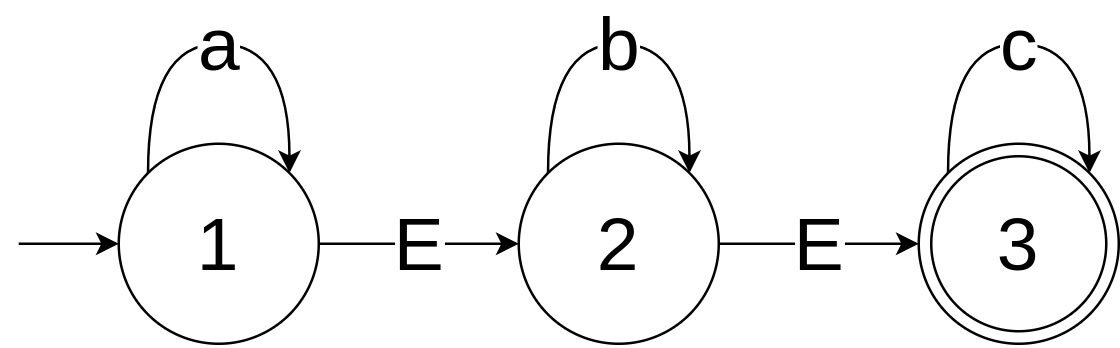
\includegraphics[width=2in]{../EXP5/diagram-ques.png}
	\caption{$\epsilon$-NFA}
\end{figure}

\begin{figure}[H]
	\centering
	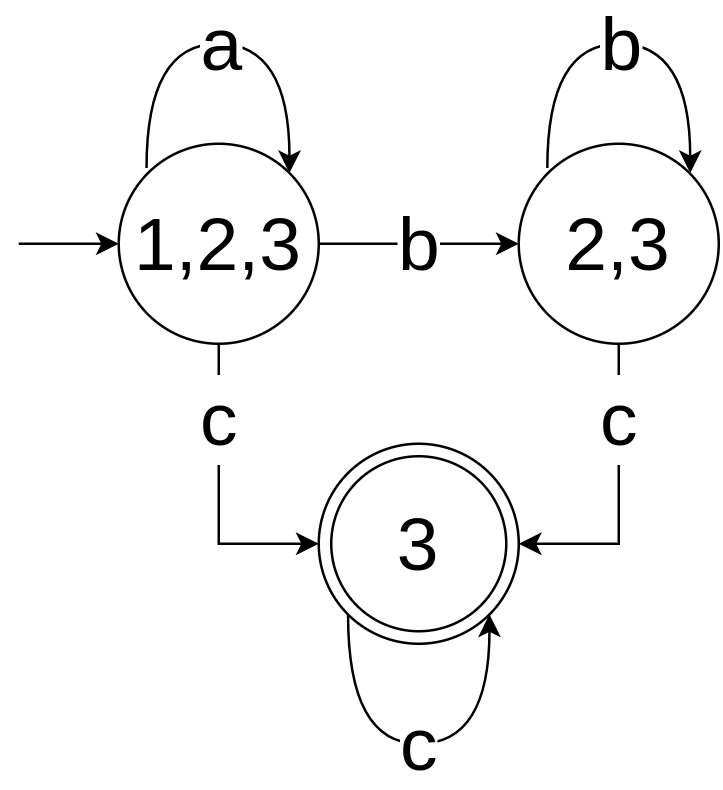
\includegraphics[height=2in]{../EXP5/diagram-ans.png}
	\caption{New NFA}
\end{figure}

\section{Python-Program}
\lstinputlisting[style=CStyle,language=python]{../EXP5/E-NFA_to_NFA.py}

\section{Output}
\lstinputlisting[style=plain]{../EXP5/output.txt}

\section{Result}
The program compiled successfully and converted $\epsilon$-NFA to NFA.
\end{document}
